\definecolor{ttqqcc}{rgb}{0.33,0.33,0.33}
%dash pattern=on 5pt off 2pt
%[fill = white, rounded corners = 4pt, inner sep = 1pt]
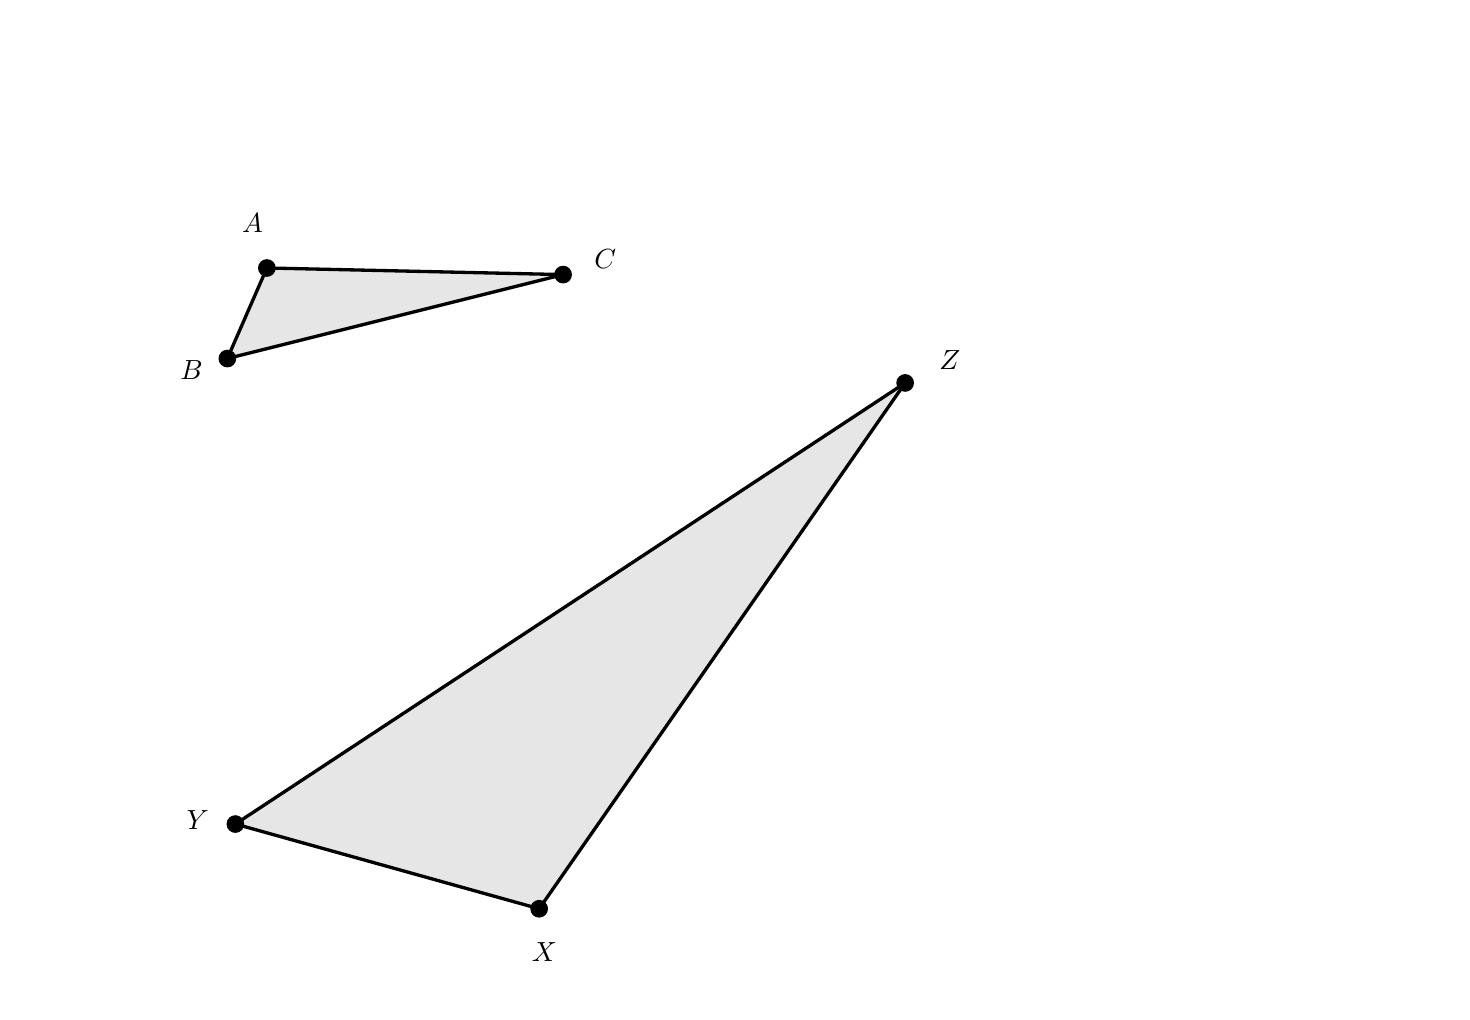
\begin{tikzpicture}[scale = 0.2]
    \clip(-20.65,-28.57) rectangle (69.12,32.66);
    \fill[line width=0pt,color=ttqqcc,fill=ttqqcc,fill opacity=0.15] (-5.46,17.4) -- (-7.97,11.65) -- (13.35,16.98) -- cycle;
    \fill[line width=0pt,color=ttqqcc,fill=ttqqcc,fill opacity=0.15] (11.83,-23.29) -- (-7.46,-17.91) -- (35.07,10.1) -- cycle;
    \draw [line width=1.2pt] (-5.46,17.4)-- (-7.97,11.65);
    \draw [line width=1.2pt] (-7.97,11.65)-- (13.35,16.98);
    \draw [line width=1.2pt] (13.35,16.98)-- (-5.46,17.4);
    \draw [line width=1.2pt] (11.83,-23.29)-- (-7.46,-17.91);
    \draw [line width=1.2pt] (-7.46,-17.91)-- (35.07,10.1);
    \draw [line width=1.2pt] (35.07,10.1)-- (11.83,-23.29);
    \begin{scriptsize}
        \normalsize
        \fill [color=black] (-7.97,11.65) circle (16pt);
        \draw[color=black] (-10.25,10.92) node {$B$};
        \fill [color=black] (13.35,16.98) circle (16pt);
        \draw[color=black] (16.03,17.99) node {$C$};
        \fill [color=black] (-5.46,17.4) circle (16pt);
        \draw[color=black] (-6.38,20.25) node {$A$};
        \fill [color=black] (11.83,-23.29) circle (16pt);
        \draw[color=black] (12.16,-26.03) node {$X$};
        \fill [color=black] (-7.46,-17.91) circle (16pt);
        \draw[color=black] (-9.85,-17.63) node {$Y$};
        \fill [color=black] (35.07,10.1) circle (16pt);
        \draw[color=black] (37.91,11.58) node {$Z$};
    \end{scriptsize}
\end{tikzpicture}